%%%%%%%%%%%%%%%%%%%%%%%%%%%%%%%%%%%%%%%%%%%%%%%%%%%%%%%%%%%%%%%%%%%%%%%%%%%%%
%%%
%%% File: utthesis2.doc, version 2.0jab, February 2002
%%%
%%% Based on: utthesis.doc, version 2.0, January 1995
%%% =============================================
%%% Copyright (c) 1995 by Dinesh Das.  All rights reserved.
%%% This file is free and can be modified or distributed as long as
%%% you meet the following conditions:
%%%
%%% (1) This copyright notice is kept intact on all modified copies.
%%% (2) If you modify this file, you MUST NOT use the original file name.
%%%
%%% This file contains a template that can be used with the package
%%% utthesis.sty and LaTeX2e to produce a thesis that meets the requirements
%%% of the Graduate School of The University of Texas at Austin.
%%%
%%% All of the commands defined by utthesis.sty have default values (see
%%% the file utthesis.sty for these values).  Thus, theoretically, you
%%% don't need to define values for any of them; you can run this file
%%% through LaTeX2e and produce an acceptable thesis, without any text.
%%% However, you probably want to set at least some of the macros (like
%%% \thesisauthor).  In that case, replace "..." with appropriate values,
%%% and uncomment the line (by removing the leading %'s).
%%%
%%%%%%%%%%%%%%%%%%%%%%%%%%%%%%%%%%%%%%%%%%%%%%%%%%%%%%%%%%%%%%%%%%%%%%%%%%%%%

\documentclass[a4paper, 12pt, oneside]{report}         %% LaTeX2e document.
\usepackage {tcdthesis}              %% Preamble.

\usepackage{hyperref} %This is for the cool links to parts of dissertation
\usepackage{epsfig}
\usepackage{amsmath}

\usepackage{url}


\mastersthesis                     %% Uncomment one of these; if you don't
% \phdthesis                         %% use either, the default is \phdthesis.

\thesisdraft                       %% Uncomment this if you want a draft
                                     %% version; this will print a timestamp
                                     %% on each page of your thesis.

\leftchapter                       %% Uncomment one of these if you want
%\centerchapter                      %% left-justified, centered or
% \rightchapter                      %% right-justified chapter headings.
                                     %% Chapter headings includes the
                                     %% Contents, Acknowledgments, Lists
                                     %% of Tables and Figures and the Vita.
                                     %% The default is \centerchapter.

% \singlespace                       %% Uncomment one of these if you want
\oneandhalfspace                   %% single-spacing, space-and-a-half
% \doublespace                       %% or double-spacing; the default is
                                     %% \oneandhalfspace, which is the
                                     %% minimum spacing accepted by the
                                     %% Graduate School.

\renewcommand{\thesisauthor}{Jonathan Frawley}            %% Your official UT name.
\renewcommand{\thesismonth}{August}                  %% Your month of graduation.
\renewcommand{\thesisyear}{2011}                      %% Your year of graduation.
\renewcommand{\thesistitle}{Procedural Content Generation of Indoor Environments for WebGL}            %% The title of your thesis; use mixed-case.
\renewcommand{\thesisauthorpreviousdegrees}{B.A(mod) in Computer Science}  %% Your previous degrees, abbreviated; separate multiple degrees by commas.
\renewcommand{\thesissupervisor}{Dr. John Dingliana}      %% Your thesis supervisor; use mixed-case and don't use any titles or degrees.
% \renewcommand{\thesiscosupervisor}{}                %% Your PhD. thesis co-supervisor; if any.

% \renewcommand{\thesiscommitteemembera}{}
% \renewcommand{\thesiscommitteememberb}{}
% \renewcommand{\thesiscommitteememberc}{}
% \renewcommand{\thesiscommitteememberd}{}
% \renewcommand{\thesiscommitteemembere}{}
% \renewcommand{\thesiscommitteememberf}{}
% \renewcommand{\thesiscommitteememberg}{}
% \renewcommand{\thesiscommitteememberh}{}
% \renewcommand{\thesiscommitteememberi}{}


\renewcommand{\thesisauthoraddress}{Trinity College Dublin}

\renewcommand{\thesisdedication}{...}     %% Your dedication, if you have one; use "\\" for linebreaks.


%%%%%%%%%%%%%%%%%%%%%%%%%%%%%%%%%%%%%%%%%%%%%%%%%%%%%%%%%%%%%%%%%%%%%%%%%%%%%
%%%
%%% The following commands are all optional, but useful if your requirements
%%% are different from the default values in utthesis.sty.  To use them,
%%% simply uncomment (remove the leading %) the line(s).

% \renewcommand{\thesiscommitteesize}{...}
                                     %% Uncomment this only if your thesis
                                     %% committee does NOT have 5 members
                                     %% for \phdthesis or 2 for \mastersthesis.
                                     %% Replace the "..." with the correct
                                     %% number of members.

\renewcommand{\thesisdegree}{Master of Science in Computer Science}  
                                     %% default is "DOCTOR OF PHILOSOPHY"
                                     %% for \phdthesis or "MASTER OF ARTS"
                                     %% for \mastersthesis.  Provide the
                                     %% correct FULL OFFICIAL name of
                                     %% the degree.

\renewcommand{\thesisdegreeabbreviation}{M.Sc.}
                                     %% Use this if you also use the above
                                     %% command; provide the OFFICIAL
                                     %% abbreviation of your thesis degree.
\renewcommand{\thesistype}{Dissertation}    %% Use this ONLY if your thesis type
                                     %% is NOT "Thesis" for \phdthesis
                                     %% or \mastersthesis.
                                     %% Provide the OFFICIAL type of the
                                     %% thesis; use mixed-case.

% \renewcommand{\thesistypist}{...}  %% Use this to specify the name of
                                     %% the thesis typist if it is anything
                                     %% other than "the author".

%%%
%%%%%%%%%%%%%%%%%%%%%%%%%%%%%%%%%%%%%%%%%%%%%%%%%%%%%%%%%%%%%%%%%%%%%%%%%%%%%



\begin{document}                                  %% BEGIN THE DOCUMENT

\thesistitlepage                                  %% Generate the title page.

\thesisdeclarationpage                %% Generate the declaration page.

\thesispermissionpage                 %% Generate the copyright permission page

%\thesisdedicationpage                             %% Generate the dedication page.

\begin{thesisacknowledgments}                     %% Use this to write your
...ACKNOWLEDGMENTS...                          %% acknowledgments; it can be anything
\end{thesisacknowledgments}                       %% allowed in LaTeX2e par-mode.

\begin{thesisabstract}
WebGL enables a new generation of web applications which have access to hardware-accelerated 3D graphics.
This has impact in the area of real-time applications such as computer
games, which are seeing an increasingly large focus on web applications.

A key challenge in making 3D games for web browsers is the creation
and transmission of assets.
Large assets such as meshes and textures, characteristic
of most modern AAA games, present a challenge for web browsers
which typically work with small data sets.

Procedural content generation involves the generation of
assets using mathematical formulae.
The benefit of doing this is that assets do not have to be
physically stored or loaded, but are generated by the application
itself.
Games such as .kkrieger do this successfully to create scenes similar in quality to modern titles such as Doom 3, with very small file size.

This dissertation explores the use of procedural techniques for asset generation in WebGL for indoor environments.
3D geometric information of the areas of a building are generated using 2D procedural plan generation with extrusion into 3D.
Textures are generated using procedural techniques such as bump mapping and Perlin noise.
Two sample scenes are developed of similar complexity :
One which uses procedural content generation and one which loads in assets.
The scenes are compared against other with respect to performance, aesthetic quality and ease of creation.

\end{thesisabstract}

\tableofcontents                                  %% Generate table of contents.
\listoftables                                     %% Uncomment this to generate list of tables.
\listoffigures                                    %% Uncomment this to generate list of figures.

%%
%% Include thesis chapters here...
%%
  \chapter{Introduction}



  \chapter{State Of The Art}
Today the realm of computer graphics has changed dramatically to what it was ten years ago.
Whereas 10 years ago the only devices which supported 3D graphics were either desktop computers or custom-designed computer games consoles.

On June 2007, Apple release its iPhone to the world, which included a PowerVR MBX chip~\cite{web:powervrmbx}.
An API was developed to enable mobile developers to use OpenGL on mobile applications, where resources are limited.
The OpenGL ES 1.1 API was developed which enabled the fixed function OpenGL pipeline on mobile devices~\cite{web:opengles11}.
This then evolved into the OpenGL ES 2.0 API, which allowed for programmable shaders like desktop OpenGL~\cite{web:opengles20}.
OpenGL ES 2.0 is supported by the new PowerVR SGX chip and is in current state of the art devices such as the Nokia N900 and the Apple iPhone 4~\cite{web:powervrsgx}.
This increase in power is due to an increased demand on users for games and other graphical applications on mobile devices.

As well as mobile devices gaining increased power and popularity, a similar movement is taking place at the same time in the web domain.
HTML, the markup language used for the web, is undergoing a significant review with HTML5~\cite{web:html5}.
HTML5 is an open standard for web applications which aims to replace existing plugins such as Adobe's flash which offer similar functionality.
One of the areas where flash is immensely popular is the world of online games.
This is shown by websites such as Kongregate, which have around 42,000 people playing their games at the time of writing~\cite{web:kongregate}.
Sites such as html5games~\cite{web:html5games} aims to capture this market using HTML5 as the technology.

HTML5 does not define a standard for 3D graphics, although a standard known as WebGL has been developed to fill this gap.

\section{WebGL}
WebGL is a 3D rendering API designed for the web.
WebGL is base on OpenGL ES 2.0 and offers similar functionality.
WebGL acts as a rendering context for the HTML5 canvas element~\cite{web:html5canvas}, which supports programmatic rendering in web pages using different rendering APIs.
An existing 2D rendering context also exists known as CanvasRenderingContext2D, which provides the ability to draw in 2D on web pages.

WebGL enables a new generation of web games which are 3D, rather than 2D as current web games are.
Tech demos for WebGL show advanced effects such as bump-mapping~\cite{web:webglbumpmapping} and real-time water effects~\cite{web:webglwater}.

WebGL provides a set of flexible primitives which should be applicable in any use case.
The idea is that APIs will be developed on top of WebGL to provide support for specific areas.
Indeed a list of frameworks built on top of WebGL is available on the Khronos wiki~\cite{web:webglframeworks}.

\subsection{WebGL Frameworks}
There are a variety of web frameworks to choose from nowadays.
This section will discuss a few of them and their merits for use with WebGL.

\paragraph{Javascript}
Javascript is the main language used by web browsers and is built into all modern browsers.
Javascript includes dynamic typing, objects, run-time evaluation.
Functions are first-class objects in javascript, and it is possible to have nested functions.
It uses prototype-based inheritance however, which most programmers would not be familiar with.

There are many quirks in javascript which some programmers abuse and according to Crockford~\cite{web:javascriptbadparts}
It's lack of strong typing and the leniancy of some web browsers on some javascript errors can make it difficult to troublshoot issues.

For use with webgl, the advantage is that javascript is the default language for interacting with webgl.
There are also numerous frameworks written in javascript to ease the use of webgl~\cite{web:threejs}\cite{web:copperlicht}. 

\paragraph{Coffee-script}
Coffee-script~\cite{web:coffeescript} is a language which compiles directly to javascript.
It includes classical inheritance as well as comprehensions and other features which improve upon javascript.
The output javascript passes jslint~\cite{web:jslint}, a javascript code-quality tool.

It also allows the user to use webgl natively and since it compiles to javascript, all of the existing javascript frameworks can easily be used.

\paragraph{Processing.js}
Processing.js~\cite{web:processingjs} is a framework for executing programs written in the Processing~\cite{web:processing} language in the web browser.
Processing is a java-like language for executing small programs known as ``sketches''.
The advantage to processing is that it enables quick demos to be programmed, as a lot of the details of drawing are abstracted away from the programmer.
It has support for WebGL however it does not give the programmer control over the lower-level details of optimisation which may be needed to get maximum performance from this project.

\paragraph{Gwt}
Gwt~\cite{web:gwt} is a framework for creating web applications in the Java programming language~\cite{web:java}.
The Java code is compiled to javascript as with Coffee-script.
The advantage to using java is that it is statically typed, is well-known and there are many existing tools to use with it.
The translation is not as straightforward however.
It is also difficult to use javascript libraries with Gwt, requiring the writing of a jsni wrapper~\cite{web:jsni} to communicate back and forth.

There are modules for use with webgl with Gwt.
The most mature of which is gwtgl~\cite{web:gwtgl}.
In testing this out however it is still a work-in-progress and is not stable enough to use for this project.


\section{Problems With WebGL}
%TODO:Important stuff here! 33% of demo
    >> Difficult to use large assets
    >> Based on OpenGL ES 2.0
    >> Advantages
        -> Easy delivery of applications (No need for explicit download)
    >> Disadvantages
        -> Limited feature set compared to desktop OpenGL.
  - GwtGL
  - Processing


\section{Procedural Content Generation (PCG)}
The generation of procedural content is important for many real-time applications. 
As we will see in this section it has been used to generate vast cities in real-time, the interiors of buildings and graphics effects on standard hardware.
Procedural Content Generation has the potential to 

\subsection{City Generation}
Recently, there has been much interest in the procedural generation of cities.
Ma\"{i}m et al.~\cite{maim2007populating} demonstrated how it is possible to recreate the population of historic cities using procedural techniques.
The use of procedural techniques to generate the crowds in Pompeii allowed realtime simulation with great variety in character representation.
This would not have been possible with traditional techniques.

The Metropolis project~\cite{web:metropolis} investigates the simulation of crowds in a modern city context.
Members of the crowd are modelled based on a variation of some template.
Different clothes are applied to the same templates to give the illusion of variation in the character models~\cite{mcdonnell2007pipeline}.
People are represented as agents which react to their environment~\cite{ulicny2002towards}.
In this way crowds are simulated using a variety of procedural techniques.

\begin{figure}
  \centering
    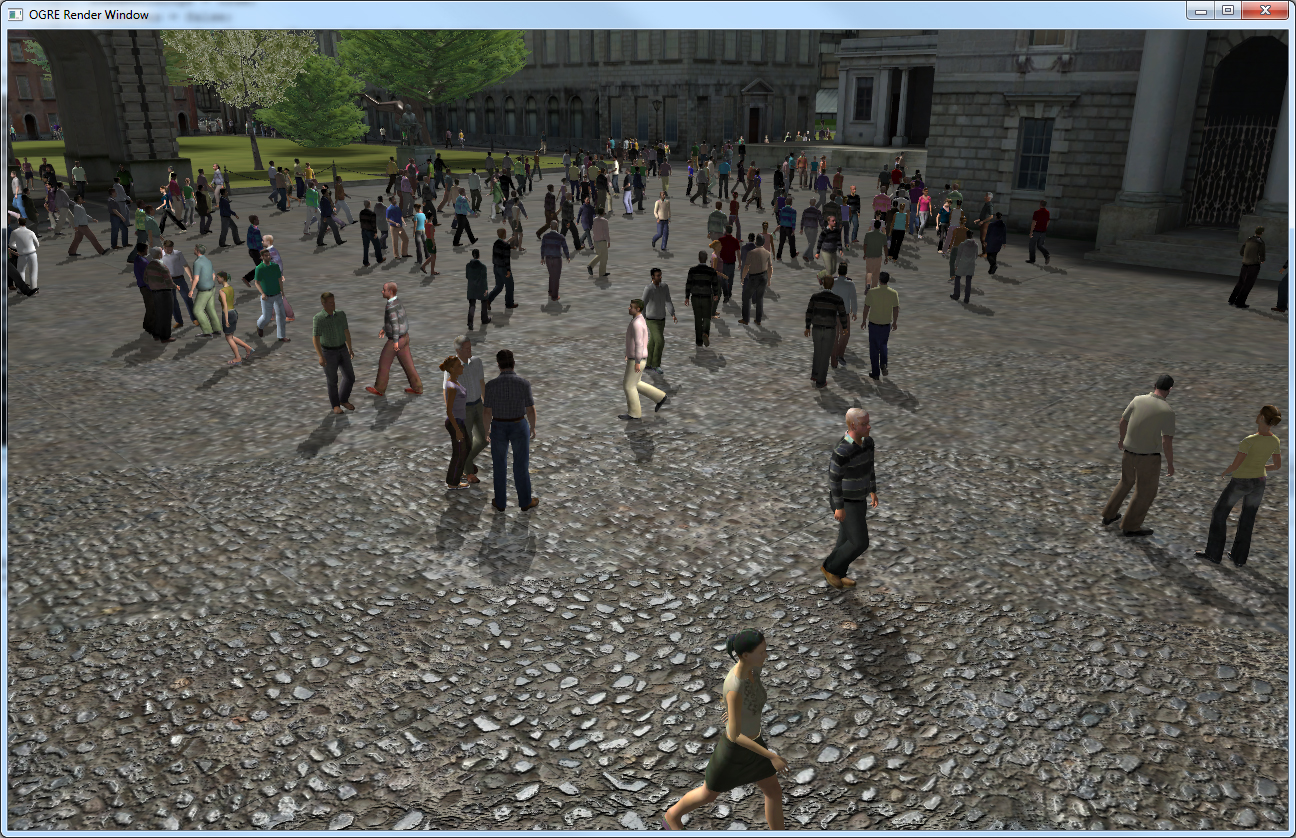
\includegraphics[width=0.7\textwidth]{images/metropolis}
  \caption{Screenshot of the Metropolis program in action}
\end{figure}

CityEngine~\cite{parish2001procedural} is an example of how procedural techniques can be applied to generates environments of great depth.
Using a combination of extended L-systems and self-sensitive L-systems, roads are generated which realistic simulate that of a target city.
Plans of buildings are generated between road segments in a recursive subdivision scheme, which discards inaccessible buildings.
The models of buildings are generated using an L-system using the bounding box of the building as the axiom of the L-system.
A technique known as \emph{layered grids} is proposed for the procedural generation of interesting textures for buildings.

\begin{figure}
  \centering
    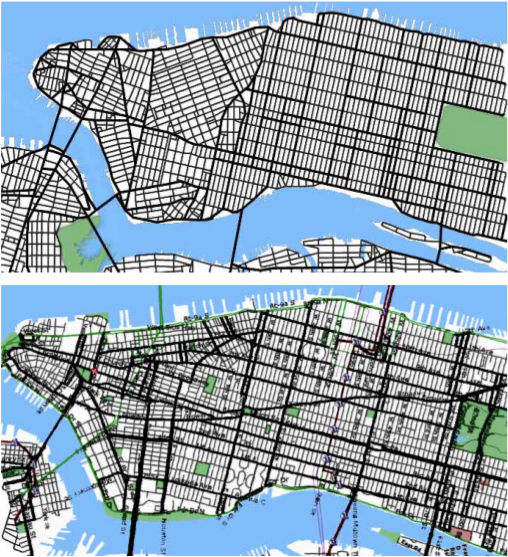
\includegraphics[width=0.7\textwidth]{images/cityengine}
  \caption{Above: Street plan generated by CityEngine. Below: Actual plan of central manhattan.}
\end{figure}


Wonka et. al present a method for automatically modelling architecture~\cite{wonka2003instant} which generates a wide range of architectural features.
A new type of design grammar known as a ``Split grammars'' is used to derive building designs.
This allows the restriction of types of allowed rules. 
These restrictions make the grammars powerful enough for the modelling of buildings.
A parameter matching system allows the user to specify multiple high-level design goals so that the output appears consistent.
Control grammars are introduced which are simple context free grammars which handle spatial ideas in an orderly way which corresponds to architectural principles.
This paper's method gives a useful insight into how architectural features may be used to further enhance the generation of buildings in a procedural way.


\subsection{Building Interiors}
CityEngine provides a method for generating the exteriors of buildings, however this project will focus on the generation of indoor environments using procedural techniques.
Greuter et al. provide methods for generating\cite{greuter2003real} floor plans of buildings in a procedural fashion.
Plans are generated by merging various polygonal shapes in a pseudo-random fashion to generate a final plan of a series of floors.
These floor plans are extruded into the 3rd axes and the outdoor buildings models are created from this.
The floors are not populated with rooms however as the indoor environments are not meant to be seen.

So et al. use wall extrusion for generating 3D indoor environments from floor plans~\cite{so1998reconstruction}.
These generated indoor environments contain rooms.
So et al. apply the technique to a CAD tool, but the technique could easily be applied to an OpenGL-based environment also.

Hahn et al present a novel approach to the generation of virtual building interiors in real-time~\cite{hahn2006persistent}.
The approach uses a lazy generation scheme which is advantageous as it means that the amount of memory used is small. 
They divide the interiors of buildings into temporary regions and built regions.
Built regions contain the final visible product of the generator and hold the geometry needed for collision detection and rendering.
Temporary regions are placeholder regions which are turned into built regions in a lazy fashion.
Temporary regions are populated when the player enters them, via a portal system.
The generation of built regions is split into stages to simplify the implementation:

\begin{enumerate}
	\item Building Setup : Anything which effects multiple floors is generated at this stage. Elevators and stairs are included as well as global textures.
	\item Floor Division : Divides the building into evenly spaced floors. Floors are then divided into 2 parts.
	\item Hallway Division : Hallways are constructed by dividing the regions around other blocks which can be rectangular loops or straight segments of hallway. 
	\item Room Cluster Division : Regions between hallways are divided into rooms. 
	\item Built Region Generation : The geometry of the room is created and it is populated with objects. This is only done if the room contains a portal.
\end{enumerate}

The oldest generated built regions are periodically deleted to control memory. 
Newly generated built regions are put into a LRU cache so that they can be easily recalled if the player moves back into the region.

\subsection{Demoscene}
The demoscene is a community of computer programmers who specialise in making impressive visual and audio effects.
There is usually an emphasis on small code size such as the 4K competitions which has the restriction on a code size of 4KB~\cite{web:demoscene4k}.
These restricted sized demos are usually referred to as Intros.

Many demoscene programmers have applied their expertise to game-related applications.
One notable example is .theprodukkt~\cite{web:theprodukkt}, who developed the .kkrieger application~\cite{web:kkrieger}.
.kkrieger displays graphics of a level comparable to Doom3 in an executable which is 96K in size.
A comparison of .kkrieger with Doom 3 can be seen in \ref{fig:kkriegerdoomcomp}.
It achieves the results seen using a variety of procedural techniques, many of which will be applicable for this project.
An example is the procedural generation of textures.
It is unfortunant however that Demoscene programmers rarely release the code that they use to produce the effects shown.
This is the case with .kkrieger also.

\begin{figure}
  \centering
  \subfloat[.kkrieger]{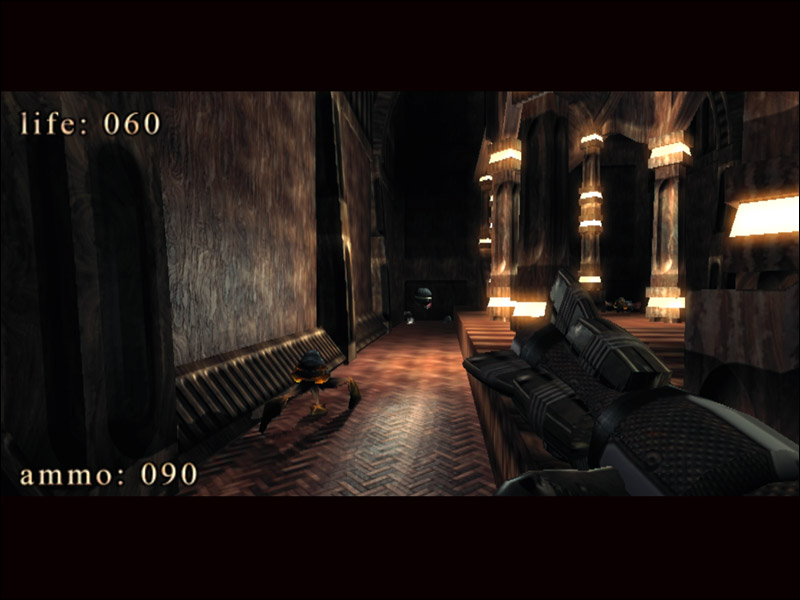
\includegraphics[width=0.5\textwidth]{images/kkrieger}}                
  \subfloat[Doom 3]{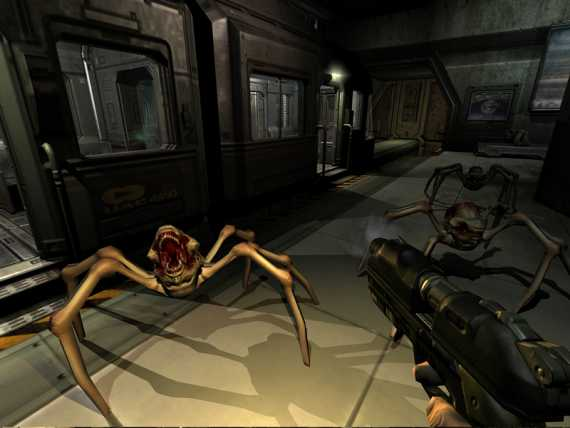
\includegraphics[width=0.5\textwidth]{images/doom3}}                
  \caption{Comparison screenshots of Doom 3 and kkrieger}
  \label{fig:kkriegerdoomcomp}
\end{figure}


  \chapter{Design}
\label{ch:design}
WebGL promises a new generation of 3D web games.
However the problem of transporting the assets over the network in an acceptable timeframe is challenging.
One way of dealing with it is to use some of the procedural content generation techniques discussed in Section~\ref{sec:pcg}.
However, how to incorporate those techniques into a new technology such as webgl is non-obvious.
We also have to keep in mind that since this is a research project, we need to be able to evaluate our results, so having a version of the application which loads in assets from the network normally as well as one which procedurally generates assets would be advantageous.

This chapter will present the design of a system which uses procedural content generation to generate the plans of buildings in WebGL.
The design presented is very general however, and can be used as a template for anyone incorporating any kind of procedural content generation into their projects on any platform.

\section{Design Goals}
\label{sec:designgoals}
The design of this project involved having a few main design goals:
\begin{itemize}
    \item Scenes which resemble a current game
    \item Ability to assess performance relative to a non-procedural version
    \item Easy to edit design program
\end{itemize}

I will now describe these design goals and how they were addressed in the context of this project.

\subsection{Scenes Resembling a Game}

This affected every aspect of the project in one way or another.
When it came to deciding on which texture effects would be implemented, perlin noise and bump mapping were chosen due to their wide use in games~\cite{web:perlingames}~\cite{kilgard2000practical}.
At all aspects of this project, realt-time interactive frame rates and loading times were seen as being necessary.

\subsection{Ability to Assess Performance}
This goal led me to the seperation of the project into two applications:
\begin{itemize}
	\item One which allows the user to design the plan and generate geometry to be output to a file
	\item One which displays the geometry using WebGL and can either procedurally generate the content on the fly or can read in the assets from files.
\end{itemize}

Two different frameworks were chosen, based on their suitability for the task.
Processing~\cite{web:processing} was chosen as the language for the design program.
Processing is written in the Java programming language, which I was already very familiar with.
Processing has a lot of built in features for displaying and drawing 2D patterns, and it was thus ideal for displaying the plan generated to the user.
It also easily allows the programmer to write information to files.

GwtGL~\cite{web:gwtgl} was chosen as the framework for the WebGL application itself.
It has the advantage that it is written in the Java programming language, compiled to javascript using the Google Web Toolkit~\cite{web:gwt} compiler.
This made code reuse possible between the main WebGL application and the design application.
In particular, the geometry generation stages were identical in code.
I would encourage anyone doing similar work to consider these frameworks.
In particular processing is a very flexible framework and is very performant.

\subsection{Intuitive Design Program}
The design program was designed so that the output could be configured by a small number of input variables.
The program is such that it should be editable by novice programmers such as artists, etc.
The input variables which can be modified are very centred around the apperance of the output.
For example the width and height of rooms in the plans are two of the parameters to the application.
Other parameters include the height on the y-axis of the projected plan in 3D.
Another parameter is the maximum number of rooms in the plan in the x and y axes.
With the modification of these parameters, it is possible to generate a variety of plans.
A few example designs are shown in Figure~\ref{fig:designapp}.

\begin{figure}
  \centering
  \subcaptionbox{Input: xRoom=3, yRoom=4, nRooms=4}{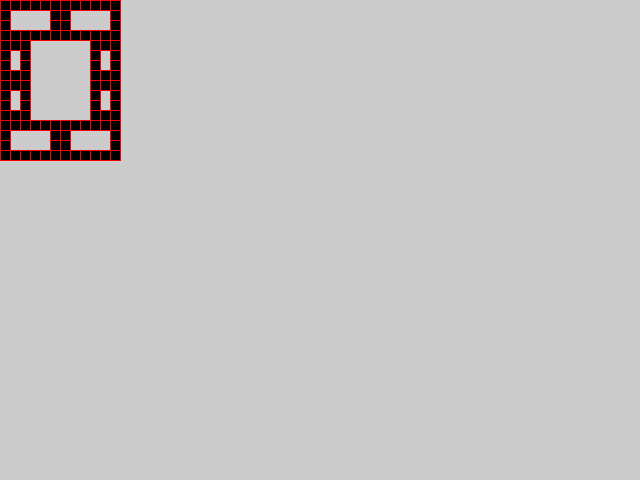
\includegraphics[width=0.4\textwidth]{images/plan/screen0}}
  \subcaptionbox{Input: xRoom=3, yRoom=4, nRooms=5}{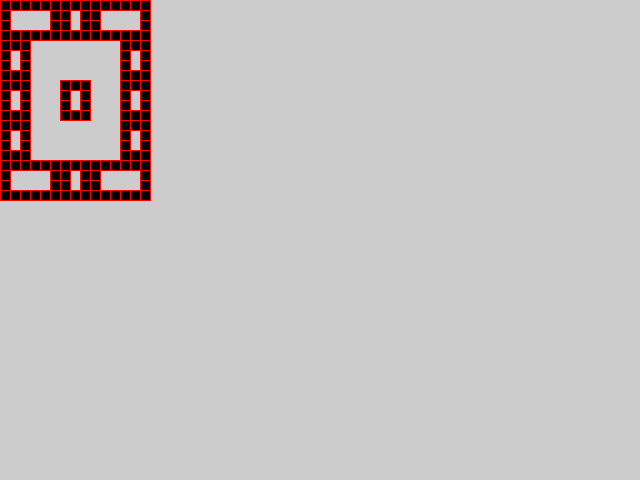
\includegraphics[width=0.4\textwidth]{images/plan/screen1}}
  \subcaptionbox{Input: xRoom=3, yRoom=5, nRooms=9}{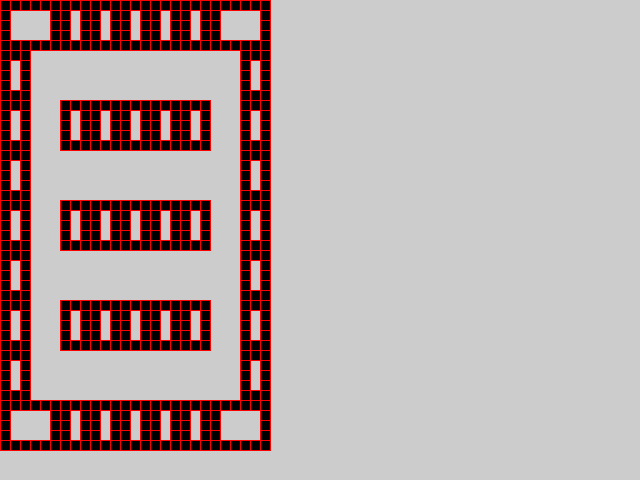
\includegraphics[width=0.4\textwidth]{images/plan/screen2}}
  \subcaptionbox{Input: xRoom=5, yRoom=3, nRooms=11}{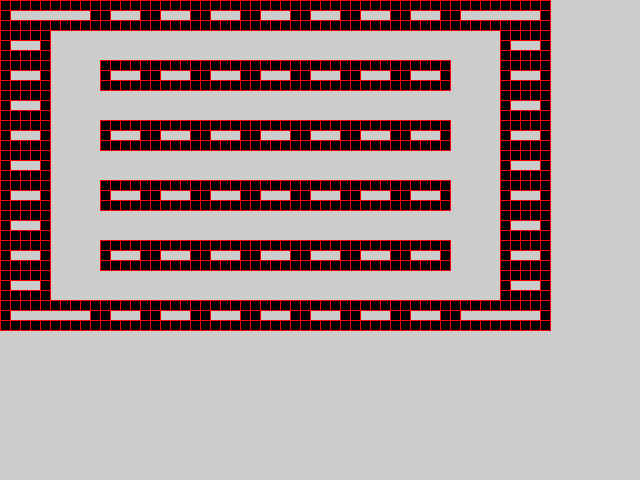
\includegraphics[width=0.4\textwidth]{images/plan/screen3}}
  \caption{Different Plans generated using the design program}
  \label{fig:designapp}
\end{figure}

\section{General Architecture}
The architecture of the system is divided into two distinct applications for the reasons described in Section~\ref{sec:designgoals}.
The general architecture is depicted in Figure~\ref{fig:sysarch}.
The architecture shows which parts of the system are shared between the 2 applications, and which parts are distinct.

I believe this architecture should hold true for any project which uses procedural content generation, though the specific methods of how how the geometry is generated will likely change from project to project.
This project is an implementation of this generic architecture and should be seen as a proof-of-concept that this architecture works in practice.
The architecture's design is based on that presented by Greuter et. al in 2003~\cite{greuter2003undiscovered}, with the main exception being that our architecture also includes texture generation explictly as part of the architecture and a design program.

The input parameters are as follows:
\begin{itemize}
	\item xRoom : The size of each room along the X-Axis
	\item yRoom : The size of each room along the Y-Axis
	\item nRooms : The number of rooms to generate in the resulting plan on each axis
\end{itemize}
These input parameters affect the way the resultant plan appears.

\begin{figure}
  \centering
  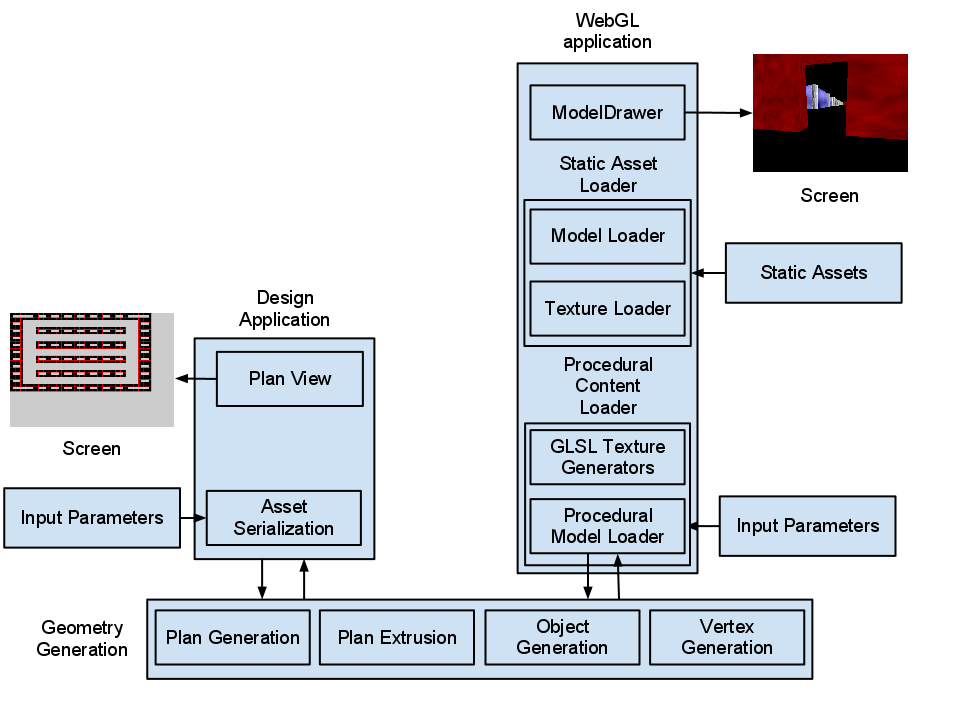
\includegraphics[width=\textwidth]{images/gwtprocArchitecture}
  \caption{System Architecture}
  \label{fig:sysarch}
\end{figure}

We will now focus our attention on both parts of this application in turn.

\subsection{Geometry Generation}
\label{sec:desgeomgen}
The phases involved in the geometry generation generation process are quite general in nature.
The plan generation phase is influenced by the input parameters.
It generates rooms in a grid-like fashion, and places other objects such as pillars in their locations also.
The Plan Extrusion process involves creating objects from the plan generated from the plan generation process.
Object generation creates objects based on certain parameters.
For instance the pillars are generated to defined level by progressive refinement.
Vertex Generation involves creating a collection of vertex objects which have enough information to render.

\subsection{Design Application}
The design application's purpose is to take a number of parameters as input and to output geometry in the form of files which can be read by the WebGL application.
The vertices for the rooms and other objects are retrieved from the Geometry Generation process.
The rooms are then drawn to the screen by the Plan View.
This gives the user an impression of what the resulting geometry will look like.
The Asset Serialization stage uses the Geometry Generation process described in Section~\ref{sec:desgeomgen} and converts the resultant vertices to Strings.
It then writes these strings to different output files, depending on the model being generated. 
These files can then be parsed and loaded by the WebGL Application.

\subsection{WebGL Application}
The WebGL application can either read in static assets from files or it can procedurally generate the assets, using the common Geometry Generation stages.
A flag is set in the WebGL application to indicate which version has been chosen.
If the static assets version of the application has been chosen, no procedural content generation is done - the assets are read in from files.
For textures this means loading in image files and for models it means reading files of text representing the information for the vertices.

When procedural content generation has been chosen it uses common Geometry Generation phases to get the vertex information for the models.
The procedural model loader is influenced by the input parameters and in this way models with varying complexity and size can be generated.

  \chapter{Implementation}

 - Details of the the codebase.
    >> UML
    >> Seperation of procedural and non-procedural
    >> Processing application vs GwtGL demo

\section{Geometry Generation}

 - Plan generation
 - Extrusion

 - Problems:
    >> Time constraints
        -> No time to implement all of the plan generation
        -> No progressive meshes

\section{Texture Generation}
 - Perlin Noise
 - Bump mapping
 - Lighting

 - Problems:
    >> WebGL current limitations.
        -> No noise() function
        -> OpenGL ES 2.0 extensions are generally not supported yet.

  \chapter{Evaluation}
\label{ch:evaluation}
The implementation of the prototype was described in Chapter~\ref{ch:impl}.
This chapter is concerned with testing the procedural version of the WebGL application vs. a non-procedural version, where static assets were used.

When we speak of performance we are considering initialisation time only, as when running the scenes are identical and will perform identically.
To accurately determine the performance of both versions, the codebases were diverged.
This is necessary as for the static assets version, the assets are included in the javascript sent to the client.
Including these in the procedurally generated version would cause unnecessary slowdown in initialisation.
Also, the procedurally generated version has many shaders which are unnecessary for the static assets version and would affect its initialisation time.
We present an explanation of how the performance tests were setup, present the results of the performance test.

We will then compare the output of the program to comparable WebGL games to assess the aesthetic complexity of the scenes created.

\section{Local Performance Test Setup - Static Assets}
The static assets version of the codebase was setup to read in 6 different textures, one for each of the objects in the scene.
Each texture is 1024x1024 in resolution, which is a pretty standard texture size for games theses days.
Popular texture sites such as Mayang's textures have textures with resolution 1600x1200 ~\cite{web:mayangtex}, so we think 1024x1024 is very reasonable.
Since the objects in the scene vary greatly in size it would be possible to texture some objects such as pillars with smaller textures, however this was not done.
All objects use the same shaders to render them, namely the fragment shader in Listing~\ref{lst:withtexfrag} and the vertex shader in Listing~\ref{lst:withtexvert}.
The author originally wanted to create a separate bump mapping shader, where the normal information was retrieved from a texture image, however time prevented this.

Once the textures are loaded, the models are retrieved from the assets generated from the design program.
This is described in Section~\ref{sec:staticassetimpl}, and basically involves reading line by line the models and creating WebGL buffers from these, with which we can draw the information.

In our initialisation tests, we also include one call to the ``ModelDrawer.draw()'' function for each, as this will compile and link the shaders.
This is important to consider as compiling and linking shaders takes time, and longer shaders will take longer to compile.
Therefore, for a fair comparison of both procedural and the non-procedural versions, we must make an initial draw call.

\section{Local Performance Test Setup - Procedural Content Generation}
The procedurally generated content version of the codebase does not read in any textures of models, but generates them entirely from scratch.
The process is described in detail in Section~\ref{sec:procgen}, but we will describe here the performance impact of the code executed.

Firstly, what is done is the geometry generation phase is called.
This includes plan generation, plan extrusion, object generation and vertex generation.
There is very little overhead here, all that is required is to set up a few objects and the model information can be generated.
However, once the objects are created, the generation of models is very fast, as there is no expensive string parsing as with the static asset version.
This means that this version will be able to generate content in a more scalable fashion than the static asset version.

The shaders used are far more complex than the ones used for the texture generation process, so the compilation of shaders will take longer.
This is a constant time delay however which is not dependant on the size of the content generated.
It should then not affect the results of performance evaluation when the size of the content generated is increased.

\section{Local Performance Test Results}
This test involved deploying the code locally on a machine with the following specifications:

\begin{itemize}
	\item Gwt version: Gwt 2.3.0
	\item GwtGL version: GwtGL 0.9-SNAPSHOT
	\item Web Browser: Chromium 15.0.849.0 (Developer Build 0 Linux)
	\item Web Server: Apache Tomcat/5.5.33
	\item OS: Linux 3.0-ARCH x86\_64
	\item GPU: Palit Nvidia GeForce GTS 250 1024MB GDDR3 PCI-Express Graphics Card
	\item CPU: Intel Core i7 920 D0 Stepping (SLBEJ) 2.66Ghz (Nehalem)
	\item Mem: Corsair XMS3 4GB (2x2GB) DDR3 PC3-10666C9 1333MHz Triple Channel
	\item HDD: Seagate Barracuda 7200.12 500GB SATA-II 16MB Cache
\end{itemize}

We setup 5 test scenes, with increasingly large numbers of polygons in the scenes.
Each time the number of polygons is doubled.
We tested the initialisation time of the 5 scenes, with initialisation being:
\begin{itemize}
	\item Load each model (From assets or procedurally generating)
	\item Loading Textures (Only for static asset version)
	\item One draw command for each model
\end{itemize}

As we can see from the results in Figure~\ref{fig:perfresultslocal} , the time taken for the initialisation of the static asset scene increases exponentially as the size of the polygons increases.
We can also see that the initialisation time for the procedurally generated scene remains very low regardless of the input size.
We can see that it grows linearly at a very slow pace in comparison to the initialisation of the static assets.

However, for very small scenes of less than 6000 polygons, the static asset version is faster.
This is due to the fact that the procedural version has more overhead when it comes to compiling and linking shaders.
For small scenes, reading in files in a brute force fashion as is done in the static asset version is actually advantageous.

We can therefore conclude that for scenes where the complexity is greater than 6000 polygons, generating content procedurally reduces initialisation time significantly.

\begin{figure}
  \centering
  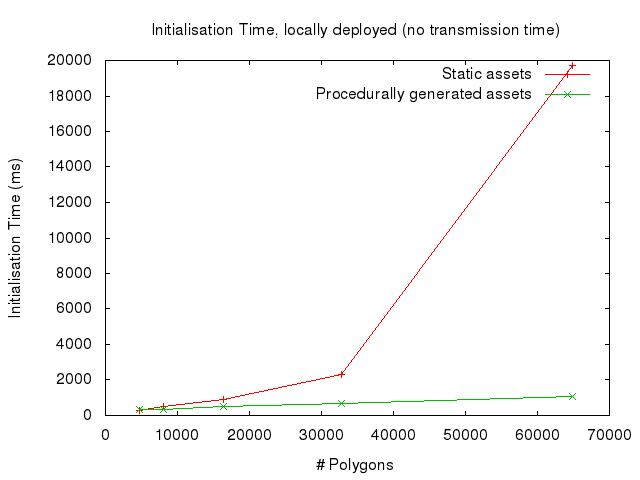
\includegraphics[width=1.0\textwidth]{images/perfresultslocal}
  \caption{Initialisation times for scenes of increasing complexity for both procedurally generated and static asset scenes}
  \label{fig:perfresultslocal}
\end{figure}

%\section{Networked Tests Performance Test Results}
%TODO:
%	>> Different connections
%	>> Different Loading times

\section{Aesthetic Complexity}
When we compare the aesthetics of this prototype, it is important to consider that the author is not an artist.
This project has merely shown that procedural effects are possible using the architecture that is presented.
It is hoped that artists will build upon the work presented here to create vastly greater effects.

That said, it compares reasonably against current generation WebGL such as is seen in Figure~\ref{fig:minevstank} where a screenshot from this demo is compared against a screenshot from TankWorld, a current WebGL Game~\cite{web:tankworld}.
As can be seen, the tankworld game contains models which are coloured uniformly.
The prototype developed in this project contains more colourful textures based on perlin noise, especially the skybox.
However, my demo does not have any lighting effects like shadowns that TankWorld has, but it does have bump mapping which TankWorld does not have.

It should be said that although this prototype does not present graphically everything that procedural generation can offer, it does compare reasonably against modern WebGL games.

\begin{figure}
  \centering
  \subcaptionbox{My Solution}{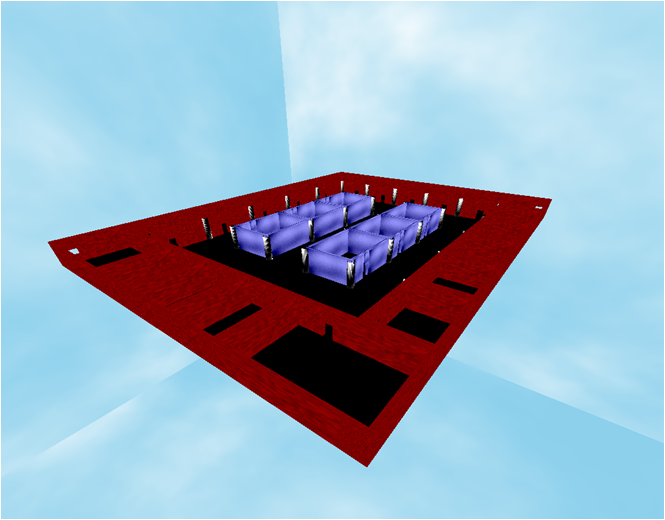
\includegraphics[width=0.5\textwidth]{images/procgl}}
  \subcaptionbox{TankWorld WebGL Game}{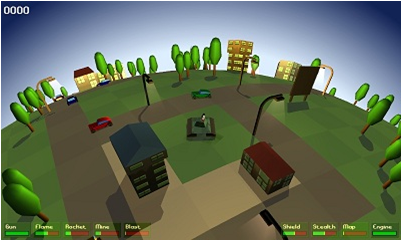
\includegraphics[width=0.5\textwidth]{images/tankworld}}
  \caption{Comparison screenshots from my prototype and a screenshot from TankWorld, a current WebGL game.}
  \label{fig:minevstank}
\end{figure}

\section{Design Program Simplicity}
\label{sec:designsimplicity}
As shown in Figure~\ref{fig:designapp}, a wide variety of scenes can be generated by changing a small number of parameters.
However to add new models it is required to create a subclass of the Entity subclass and implement the necessary functions.
This should be relatively straightforward for anyone with a knowledge of Java or Object Oriented programming, as Processing is a simple framework to use.

To create compound models, the user does not need to create new classes however, they can use the existing primitives which exist.
An interactive Gui would help with this, but there is no reason why objects like chairs, desks, shelves, etc. cannot be implemented as a combination of cuboids and cylinders.
Indeed this is an area of future work for this project.

\section{Extensibility}
Project extensibility is a big factor in everything that was accomplished in this project.
This is the first framework for procedural content generation for WebGL that the author is aware of.
It is also highly generic and it could easily be ported to desktop OpenGL or OpenGL ES 2.0 on mobile with little effort.

Nearly every part of the codebase is highly extensible.
Indeed writing new shaders is very simple, we simply need to write them and include them in the maven project and reference them in the model we want to use them for.
As said in Section~\ref{sec:designsimplicity} to extend models we simply subclass the Entity and come up with some way of generating the quads that are needed.
The entity class already has a lot of useful functions for generating models such as cuboids, so it would be trivial to create new models using these methods.

\section{Research Contribution}
The author believes what is offered here is more than just an implementation of procedural techniques in WebGL.
We have presented a generic framework for generating procedural content in WebGL.
The incorporation of both geometric and texture generation into a unified pipeline is unique in this project.

The sample programs created and tested are proof of the utility of this framework.
It also acts as a proof of concept that procedural content generation can be of benefit to anyone implementing games on this new platform, especially the vastly decreased loading times which players will experience with procedurally generated content over loading static assets.

  \chapter{Conclusions And Further Work}
\label{ch:conclusions}
This thesis has presented a generic framework for the generation of procedural content in computer graphics applications.
The emphasis has been placed on interactive applications such as games which require as little initial load time as possible.

An example application was developed which implemented the generic framework and performance analysis was performed against it and another application which loaded in meshes manually.
Using identical scenes, the two applications were tested against each other with the initialisation time of the procedurally generated version scaling much better with the amount of triangles in the scene.

This thesis has set out to outline the best practices for implementing procedural content generation in WebGL and to also prove the effectiveness of these practices with an example.
The preceding chapters have outlined the design and implementation of such a prototype.

It is hoped that this work paves the way for future researchers to develop procedural content generation in their applications, and to use the generic framework presented as their base.

\section{Further Work}
Work on improving the usability and interactivity of the design program to ensure its use by artists would be highly useful.

More advanced plan generation is one possible future avenue for developers.
At the moment there is no accepted best method for generating indoor plans of buildings of a set size.
I believe any future work needs to take account of contextual information as CityEngine does~\cite{parish2001procedural}.
Some method which takes account of factors such as population density, fire exits, hallway access, stairs access, etc. would be advantageous to generating arbitrary buildings.
To implement more advanced plan generation is possible with this prototype, and the design program can be used to help in the design.

There is a lot of work that could be done on providing more advanced effects such as realistic wood or rusting effects which were not examined due to time constraints.
Also some effects such as per-fragment lighting and shadow mapping could be looked at to further enhance the realism of scenes.

Progressive meshes~\cite{hoppe1996progressive} is a method for representing models in an efficient, loss-less, continuous-resolution way.
It would be useful to examine how progressive meshes could be used as another option for developers to generate meshes.

Developers for other low-power platforms such as mobile devices could use the information from this thesis to generate procedural content for their games.

An optimisation which could be examined is the generation of geometry on the GPU using GPGPU techniques.
Since WebGL gives access to the GPU, there is no reason why shaders could not be used to generate geometry in a very scalable fashion.

%   \include{chapter3}
%   \include{chapter4}
%   \include{chapter5}


\addcontentsline {toc}{chapter}{Appendices}       %% Force Appendices to appear in contents
\begin{appendix}
 \chapter*{Appendix}

...

% \include{appendix2}
\end{appendix}


%\addcontentsline {toc}{chapter}{Bibliography}     %% Force Bibliography to appear in contents

%\begin{thebibliography}{ieeetr}                   %% Start your bibliography here; you can
%\bibliography{refs}                               %% also use the \bibliography command
%\end{thebibliography}                             %% to generate your bibliography.


\end{document}                                    %% END THE DOCUMENT
